\documentclass[a4paper, parskip=full]{scrartcl}
\usepackage[top=3cm, bottom=3.5cm, left=3cm, right=3cm]{geometry}
\usepackage[utf8]{inputenc} % use utf8 file encoding for TeX sources
\usepackage[LGR,T1]{fontenc}    % avoid garbled Unicode text in pdf
\usepackage[german]{babel}  % german hyphenation, quotes, etc
\usepackage{graphicx}       % provides commands for including figures
\usepackage[export]{adjustbox}
\usepackage{csquotes}       % provides \enquote{} macro for "quotes"
\usepackage{hyperref}       % detailed hyperlink/pdf configuration
\usepackage{color}
\usepackage{tcolorbox}
\usepackage{hyperref}
\usepackage{tabu}			% provides tables
\usepackage{listings}
\usepackage{xcolor}
\usepackage[nonumberlist]{glossaries}     % provides glossary commands
\hypersetup{                % ‘texdoc hyperref‘ for options
  pdftitle={Entwurf},
  pdfauthor={Anna Csurkó, Jona Enzinger, Yannik Schmid, Jonas Zoll},
}
\graphicspath{{./figures/}} % Setting the graphicspath

\newcounter{counter}[section]
\setcounter{counter}{10}

\lstdefinelanguage{json}{
    basicstyle=\normalfont\ttfamily,
    numbers=left,
    numberstyle=\scriptsize,
    stepnumber=1,
    numbersep=8pt,
    showstringspaces=false,
    breaklines=true,
    frame=lines,
    backgroundcolor=\color{background},
    literate=
     *{0}{{{\color{numb}0}}}{1}
      {1}{{{\color{numb}1}}}{1}
      {2}{{{\color{numb}2}}}{1}
      {3}{{{\color{numb}3}}}{1}
      {4}{{{\color{numb}4}}}{1}
      {5}{{{\color{numb}5}}}{1}
      {6}{{{\color{numb}6}}}{1}
      {7}{{{\color{numb}7}}}{1}
      {8}{{{\color{numb}8}}}{1}
      {9}{{{\color{numb}9}}}{1}
      {:}{{{\color{punct}{:}}}}{1}
      {,}{{{\color{punct}{,}}}}{1}
      {\{}{{{\color{delim}{\{}}}}{1}
      {\}}{{{\color{delim}{\}}}}}{1}
      {[}{{{\color{delim}{[}}}}{1}
      {]}{{{\color{delim}{]}}}}{1},
}

% new environment for listing requirements/product data/... with a counter
%\newenvironment{Kriterien}[1]{
%	\let\olditem\item \renewcommand\item[1][]{\olditem[/#1\thecounter /] \textbf{##1} \hfill \\
%	\addtocounter{counter}{10}} \begin{description}}
%	{\end{description}}


\title{Entwurf}
\author{Anna Csurkó, Jona Enzinger, Yannik Schmid, Jonas Zoll}
\makeatletter

\definecolor{mintgreen}{RGB}{50,161,137} % theme color of the Karlsruhe Institute of Technology (KIT)
\colorlet{punct}{red!60!black}
\definecolor{background}{HTML}{EEEEEE}
\definecolor{delim}{RGB}{20,105,176}
\colorlet{numb}{magenta!60!black}

\newenvironment{Class}[1]{
      \begin{tcolorbox}[title=#1,colbacktitle=mintgreen,colframe=mintgreen,colback=white]
  }{
      \end{tcolorbox}
  }

% header and footer
\usepackage[automark,autooneside=false,headsepline=0.5pt,footsepline=0.5pt]{scrlayer-scrpage}
\addtokomafont{headsepline}{\color{mintgreen}}
\addtokomafont{footsepline}{\color{mintgreen}}
\addtokomafont{pagehead}{\normalfont}

% delete current settings for header and footer
\clearpairofpagestyles

% display document name on the left and current section on the right
\ihead{\@title}
\ohead{\rightmark}

% load glossary entries
\makenoidxglossaries
\loadglsentries{./chapters/Glossareintraege}

% center page number
\cfoot*{\pagemark}

\begin{document}
% beginn content
\begin{titlepage}
  \centering
  
\includegraphics[width=0.5\linewidth]{KITLogo.png}\par\vspace{1cm}
	  {\scshape \bfseries Lehrstuhl für Pervasive Computing Systems\par}
	  {\scshape \bfseries Teco\par}
	  \vspace{0.25cm}
  	{\scshape Tobias Röddiger\\Dr. Paul Tremper\par}
  	\vspace{1.5cm}

    \newcommand{\HRule}{\rule{\linewidth}{0.5mm}}
    {\color{mintgreen}\HRule} \\[0.4cm]
  	{\huge \bfseries \LARGE Anwenderorientierte Nutzerschnittstelle für Luftqualitätsdaten\par}
    {\color{mintgreen}\HRule} \\[1cm]
  	\vspace{2cm}
  	{\scshape \Large Anna Csurkó\\Jona Enzinger\\Yannik Schmid\\Jonas Zoll\par}
  	\vfill

\end{titlepage}


\tableofcontents
\section{Vorwort}
Dieses Dokument modelliert die Architektur des Programms \gls{SmartAQnet}. Wir als Entwickler-Team haben den Aufbau in Typescript components und Klassen aufgeteilt. Dabei war unser Ziel, das Programm möglichst stabil, flexibel und objektorientiert zu gestalten. Zusätzlich lässt sich die Architektur sehr gut in Model, View und Controller einteilen, indem wir die Querys, das Grundgerüst und die Benutzeroberfläche gut trennen können. Für die Erstellung der Diagramme wurde PlantUML und Visual Studio Code, für die Zusammenarbeit GitHub benutzt.


\section{Architektur}

Die Grundstruktur der Webanwendung orientiert sich an der "Model View Controller"-Architektur. Die Aufteilung ind die drei Komponenten
erleichtert das Bearbeiten von Programmcode, auch im Team, und TODO noch mehr Vorteile.
\\
Die Architektur besteht aus folgende Bestandteilen:




\section{Klassenbeschreibung}

\begin{Class}{RequestClass}
    \textbf{Methoden:}
    \begin{itemize}
        \item \texttt{getLatestObservations(center: Position, radius: int, feature: Feature): Observation[]}
        \item \texttt{getStationsIn(middle: Position, radius: int): Station[]}
        \item \texttt{getHistoricalObservations(station: Station, start: Date, end: Date): Observation[]}
        \item \texttt{getHistoricalObservations(station: Station, start: Date, end: Date, frequency: Frequency, feature: Feature): Observation[]}
        
    \end{itemize}
\end{Class}
\section{Datenmodell}
\subsection{Feature}

Unterstützte Features sind in JSON Dateien definiert.
Dies ermöglicht das einfache Hinzufügen von weiteren Features und die freie Konfiguration für die Betreiber der Seite.


\begin{lstlisting}[language=json,firstnumber=1]
    {
	    "id": string,
	    "nameId": string,
	    "unitOfMeasurement": string,
	    "descriptionId": string,
	    "limit": number,
	    "defaultScale": {
			[number] : string,
			linearTransition: boolean,
	    },
	    "supportedDiagrams": string[]
    }
    
\end{lstlisting}

\begin{itemize}
	\item \texttt{id} 
	\\ Eine eindeutige Id, wird vom FROST-Server übernommen.
	\item \texttt{nameId} 
	\\ Der Schlüssel für den lokalisierten Namen des Features
	\item \texttt{unitOfMeasurement} 
	\\ Die Messeinheit des Features
	\item \texttt{descriptionId} 
	\\ Der Schlüssel für die lokalisierte Beschreibung
	\item \texttt{limit} 
	\\ Der Messwert ab dem eine Warnung ausgegeben wird
	\item \texttt{defaultScale} 
	\\ Eine Farbskala für das Feature, dient als Fallback falls keine Skala auf dem Server gefunden wird.
	\\ Bei \emph{[number] : string} ist der Schlüssel die untere Grenze für die Farbe.
	Die Farbe selbst ist in HEX codiert (bspw. '\#AAAAAA') 
\end{itemize}
\newpage
\subsection{Sprachdateien}


\begin{lstlisting}[language=json,firstnumber=1]
	{
		"id": string,
		"name": string,
		"strings": {
			[string]: string,
		}
	}
	
\end{lstlisting}

\begin{itemize}
	\item \texttt{id} 
	\\ Eine eindeutige Id für die Sprache.
	\item \texttt{name} 
	\\ Der Name der Sprache in der Sprache selbst.
	\item \texttt{strings} 
	\\ Eine Liste an Schlüsseln und der zugehörigen Zeichenkette in der Sprache.
\end{itemize}

\subsection{FrostUrl}

\begin{lstlisting}[language=json, firstnumber=1]
	{
  		"url": string
	}

\end{lstlisting}

\begin{itemize}
	\item \texttt{url}
	\\ Die Url der API eines FROST-Servers, bspw. \url{https://api.smartaq.net/v1.0/}
\end{itemize}
\section{Anhang}
\subsection{Usability Test}
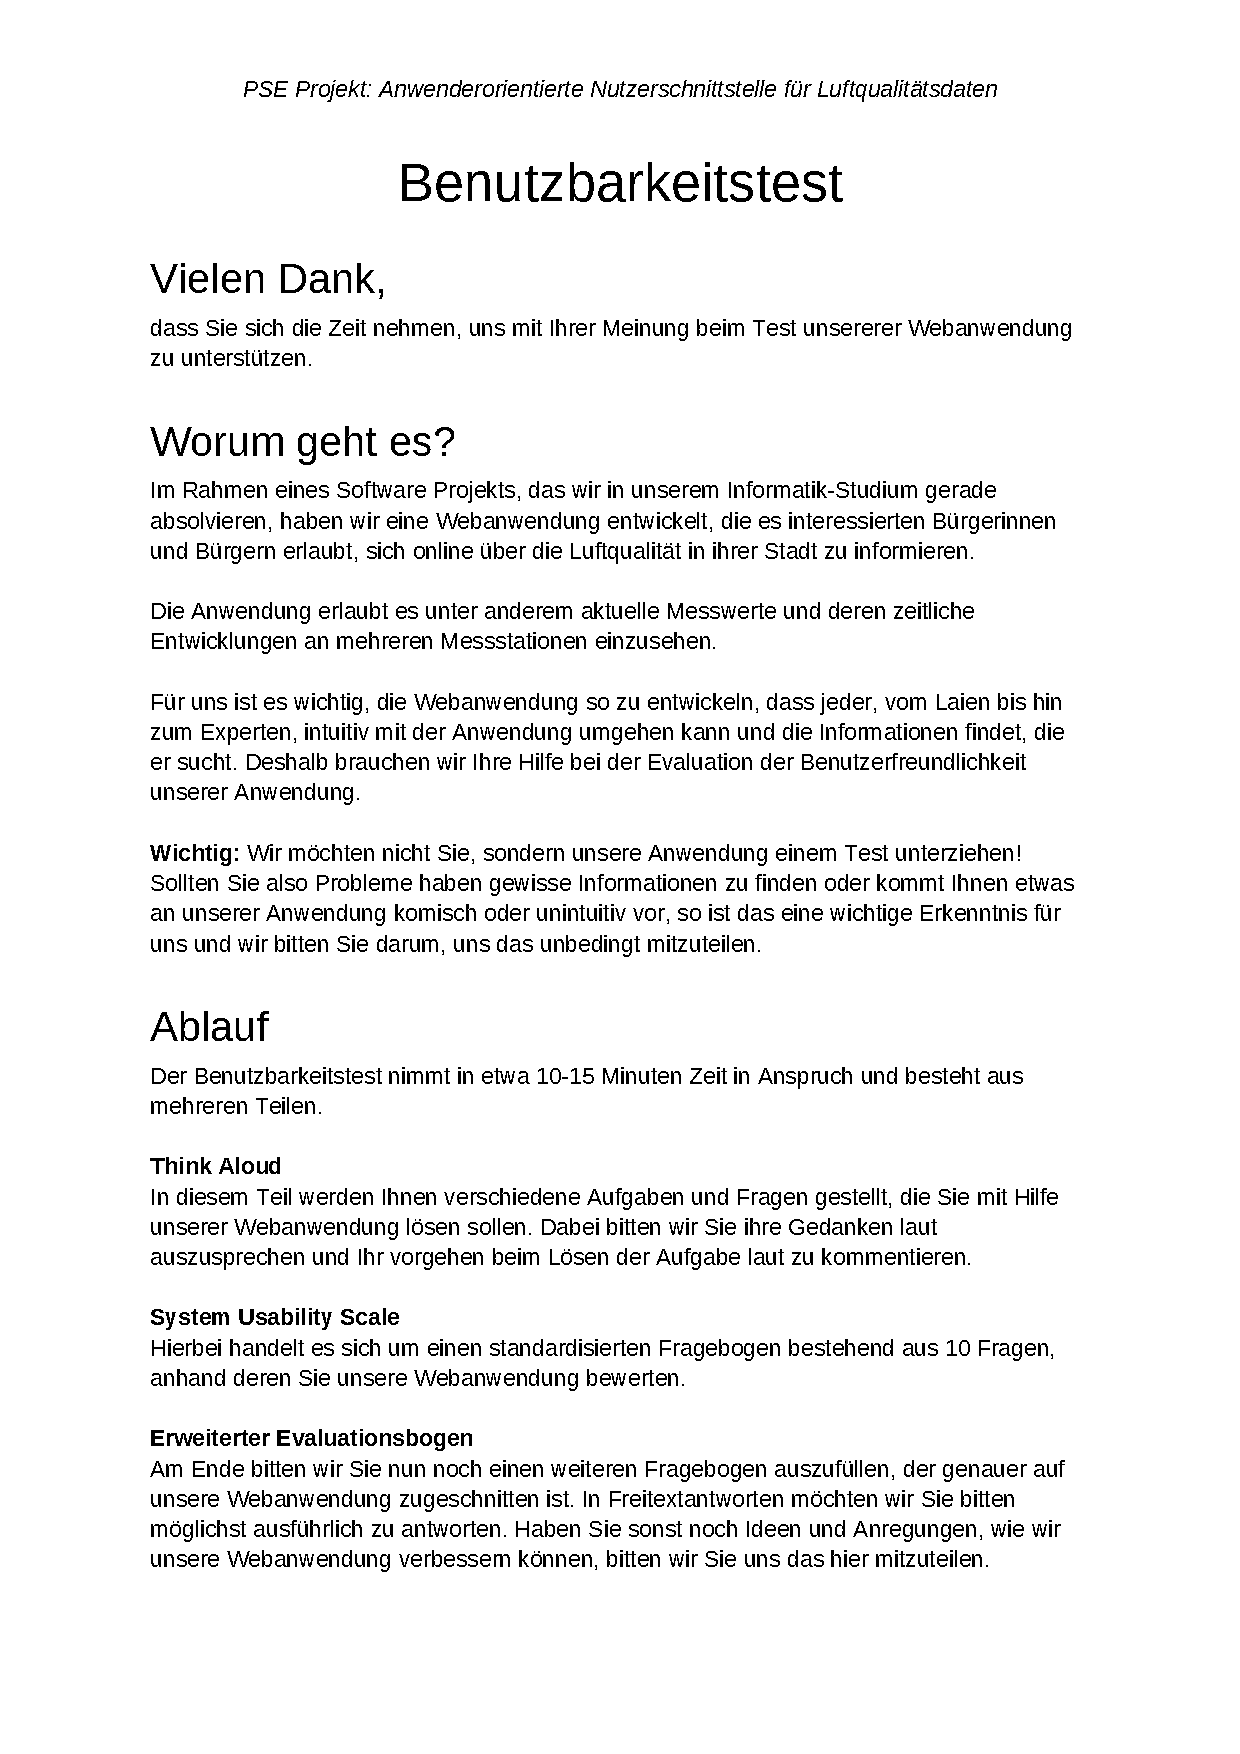
\includepdf[page=-]{./figures/usability_test.pdf}
\section{Glossar}

% automatically created glossary (compile twice to show glossary)
\glsaddall
\printnoidxglossaries

% end content
\end{document}